%----------------------------------------------------------------------------------------
%	PACKAGES AND THEMES
%----------------------------------------------------------------------------------------
\PassOptionsToPackage{table}{xcolor}
\documentclass[aspectratio=169,xcolor=dvipsnames,11pt]{beamer}
\usepackage{tikz}
\usetheme{SimplePlusAIC}
\usepackage{amsmath}
%\usepackage{animate}
%%\usepackage{hyperref}
\usepackage{cleveref}
\usepackage{caption}
\usepackage{graphicx} % Allows including images
%%\usepackage{subfig}
\usepackage{subcaption}
%\usepackage{booktabs} % Allows the use of \toprule, \midrule and  \bottomrule in tables
%\usepackage{svg} %allows using svg figures
%\usepackage{makecell}
%\usepackage{multirow}
%\usepackage{appendixnumberbeamer}
%\usepackage{wrapfig}
%\usepackage{verbatim}
%\usepackage{tcolorbox}
%%\usepackage[dvipsnames]{xcolor}
%
%\usepackage{hhline}
%\usepackage{relsize}
%\usepackage{bm}
%%Select the Epilogue font (requires luaLatex or XeLaTex compilers)
%%\setsansfont{Epilogue}[
%%    Path=./epilogueFont/,
%%    Scale=0.9,
%%    Extension = .ttf,
%%    UprightFont=*-Regular,
%%    BoldFont=*-Bold,
%%    ItalicFont=*-Italic,
%%    BoldItalicFont=*-BoldItalic
%%    ]
%    \usefonttheme[onlymath]{serif}
%% \usepackage{ eulervm } % Euler VM as math serif font
%
%\newcommand*{\defeq}{\stackrel{\text{def}}{=}}
%\newcommand{\grad}{\nabla}
%\newcommand{\lap}{\Delta}
%\newcommand{\weaklyto}{\rightharpoonup}
%\newcommand{\weakstar}{\stackrel{*}\rightharpoonup}
%\newcommand{\cts}{\hookrightarrow}
%\newcommand{\ctsDense}{\xhookrightarrow{d}}
%\newcommand{\ctsCompact}{\xhookrightarrow{c}}
%\newcommand{\E}{\mathbb{E}}
%\newcommand{\pP}{\mathbb{P}}
%\newcommand{\R}{\mathbb{R}}
%\newcommand{\ER}{\overline{\mathbb{R}}}
%\newcommand{\cR}{\mathcal{R}}
%\newcommand{\cJ}{\mathcal{J}}
%\newcommand{\cG}{\mathcal{G}}
%\newcommand{\CVaR}{\textup{CVaR}}
%\newcommand{\D}{\textup{ d}}
\newcommand{\dd}{\mathrm{d}}
%\newcommand{\fa}{\text{for all }}
%\DeclareMathOperator*{\essinf}{\vphantom{p}ess\,inf}
%\DeclareMathOperator{\sigmoid}{expit} % a.k.a. logistic sigmoid
%
%\usepackage[ruled,vlined,algo2e]{algorithm2e}
%\crefname{algocf}{algorithm}{algorithms}
% \usepackage{caption}
%
%% Define a custom style for the box
%\usepackage{tcolorbox}  % For fancy boxes
%
%% Define a custom style for the box
%\tcbuselibrary{skins, breakable}
%\newtcolorbox[auto counter, number within=section]{roundedshadowbox}[2][]{
%    colback=white, % Background color (kept white)
%    colframe=black, % Border color
%    boxrule=0.5pt, % Border thickness
%    arc=5mm, % Rounded corners
%    shadow=true, % Drop shadow effect
%    width=\linewidth, % Full width box
%    title=#2, % Title text
%    #1 % Additional options (e.g., width override)
%}

\font\nullfont=cmr10


%----------------------------------------------------------------------------------------
%	TITLE PAGE
%----------------------------------------------------------------------------------------

\title[\quad\quad\quad LVPP Course I]{The Latent Variable Proximal Point Method I: Introduction and Preliminary Results
 } % The short title appears at the bottom of every slide, the full title is only on the title page
%\subtitle{Subtitle}

\author{\small{\bf Thomas M. Surowiec}}

\institute[T.M. Surowiec]{Department of Numerical Analysis and Scientific Computing \newline Simula Research Laboratory \newline Oslo, Norway}
% Your institution as it will appear on the bottom of every slide, maybe shorthand to save space


\date[EMS School]{ {\footnotesize 
K\'acov, Czechia, 15-20 June 2025}}
%----------------------------------------------------------------------------------------
%	PRESENTATION SLIDES
%----------------------------------------------------------------------------------------

\begin{document}

{
\setbeamertemplate{background canvas}{}
\frame{\titlepage}
}

\begin{frame}{Overview}
\tableofcontents
\end{frame}

\section{Motivation and context: Variational inequalities and PDEs}\label{sec:motivation}
%\begin{frame}{Dirichlet's Principle}
%    \begin{enumerate}
%        \item History
%            \begin{enumerate}
%                \item Who invented it, when did it get its name, etc.
%            \end{enumerate}
%        \item Modern interpretation and a first variational inequality
%            \begin{enumerate}
%                \item Derivation of a variational inequality
%                    \begin{enumerate}
%                        \item The feasible set is nonempty, closed, and convex
%                        \item Existence via direct method
%                        \item The objective function is G\^{a}teaux differentiable
%                        \item Derivation of the VI
%                    \end{enumerate}
%            \end{enumerate}
%        \item Reformulation as a variational equation
%            \begin{enumerate}
%                \item Using a clever test function
%                \item Use lifting discussion see Chouly 2023, Poisson.
%            \end{enumerate}
%    \end{enumerate}
%\end{frame}


\begin{frame}{Dirichlet's Principle}

  \begin{minipage}{0.48\textwidth}
  \begin{beamercolorbox}[rounded=true, shadow=true, wd=\textwidth]{block body}
 \textit{The solution to Poisson's equation is the minimizer of a certain energy functional.}\\
  
  \visible<2->{Early observations due to Thomson and Gau\ss.}\\
  
  \visible<3->{Riemann named it after his teacher Dirichlet.}\\
  
  \visible<4->{Hilbert justified Riemann's use of Dirichlet's principle,\\ invents the Direct Method (1900-1905).}
     \end{beamercolorbox}
    \end{minipage}\hspace*{1.75cm}
    \begin{minipage}{0.3\textwidth}
  \centering
 \begin{figure}
  \centering\vspace{1ex}
  \only<1-3>{\begin{minipage}[b]{0.45\textwidth}
    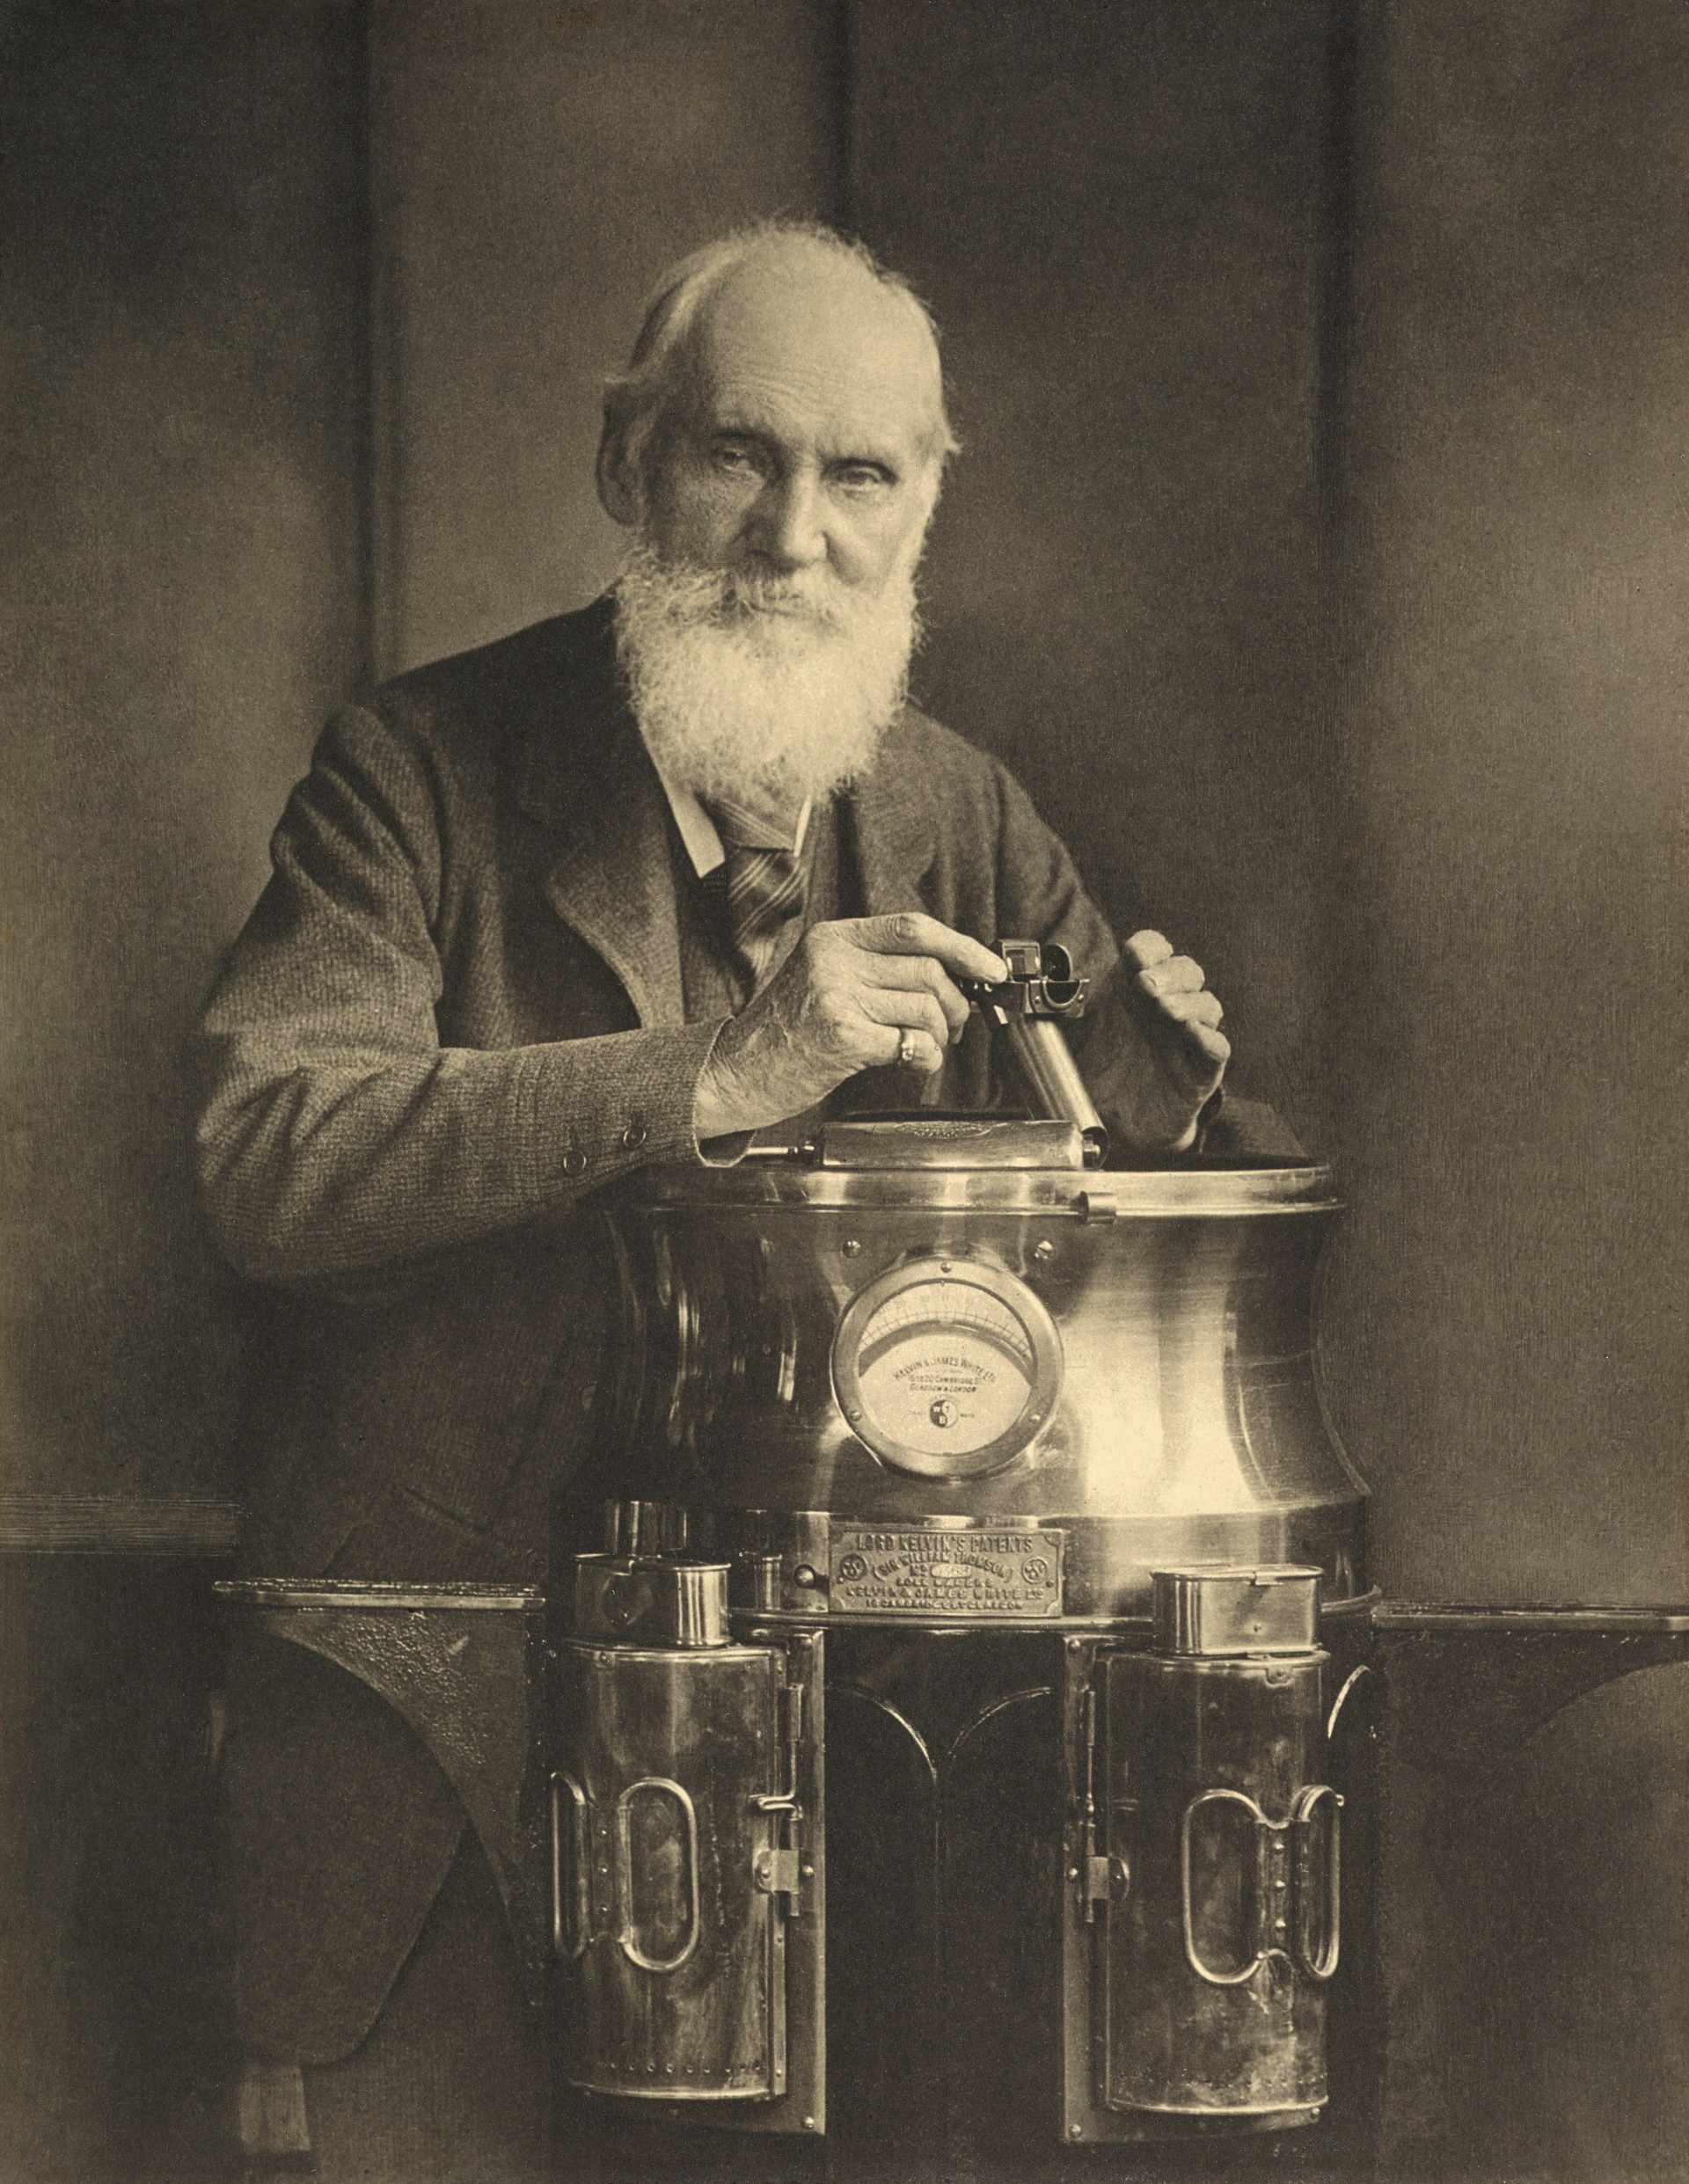
\includegraphics[width=\linewidth]{figures/kelvin.jpg}
    \captionof*{figure}{\tiny W. Thomson}
  \end{minipage}}%
   \only<4->{\begin{minipage}[b]{0.43\textwidth}
    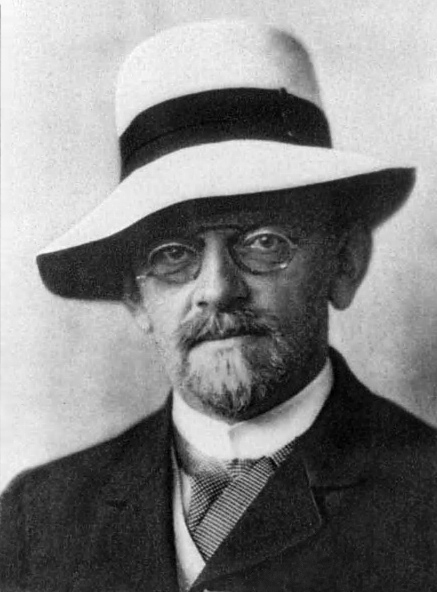
\includegraphics[width=\linewidth]{figures/Hilbert.jpg}
    \captionof*{figure}{\tiny \alert{D. Hilbert}}
  \end{minipage}}
  \hfill
  \begin{minipage}[b]{0.455\textwidth}
    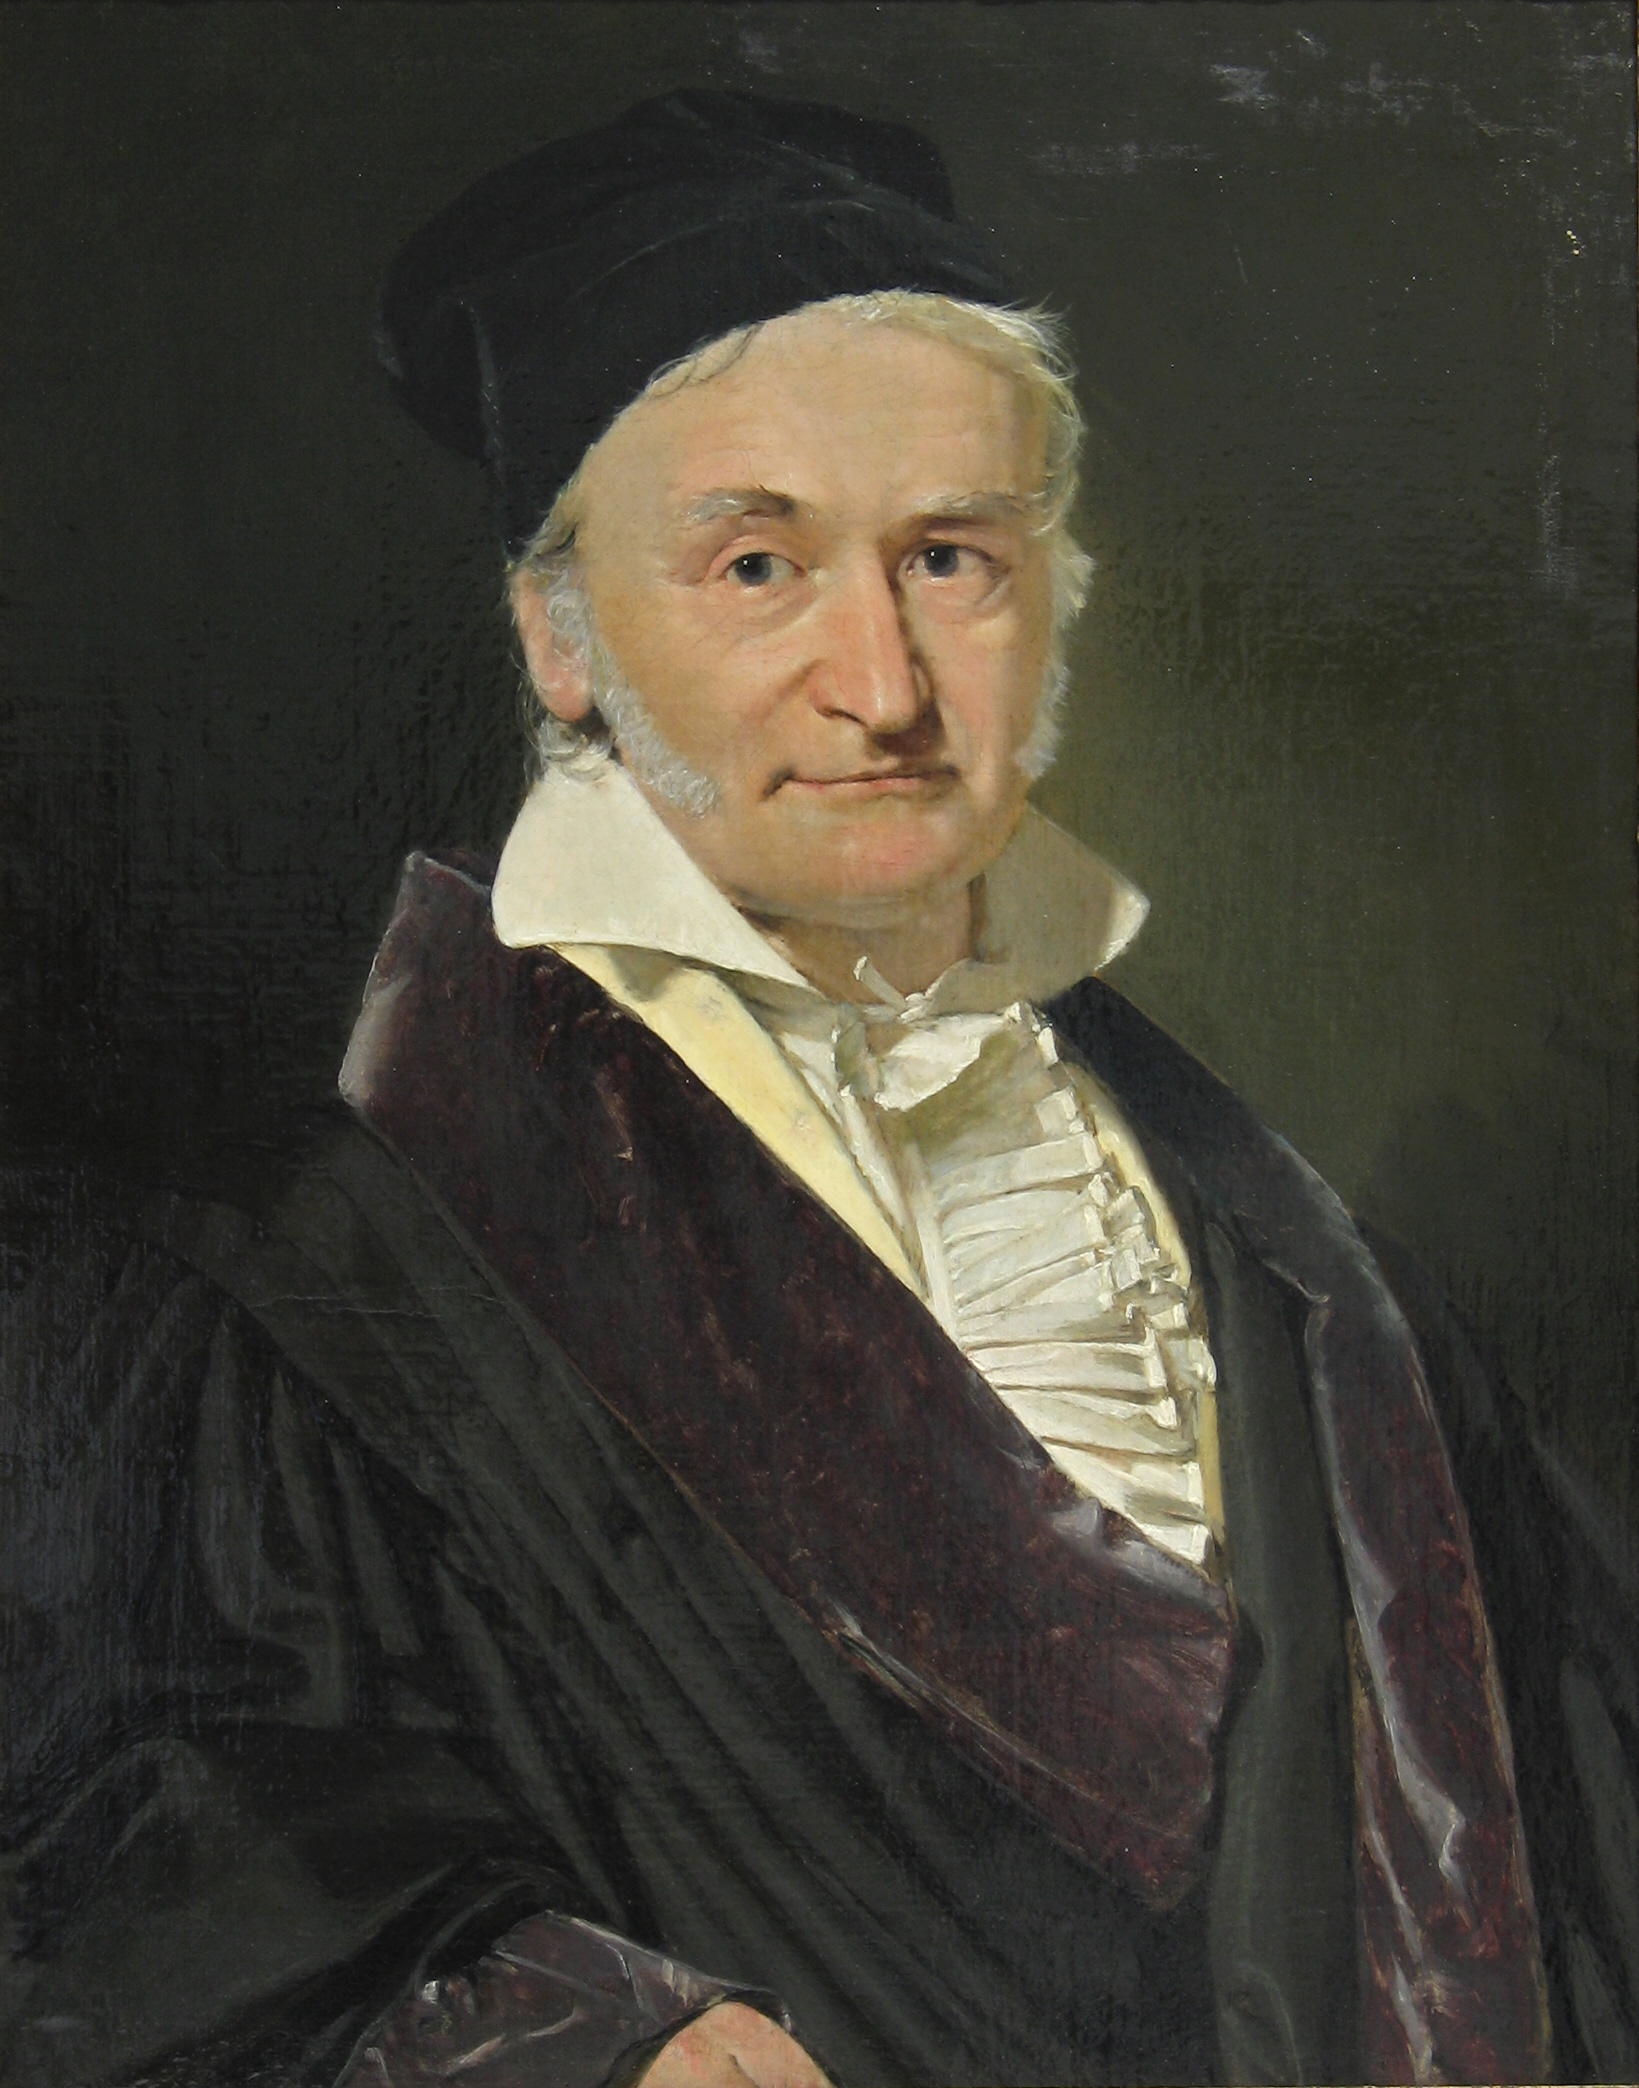
\includegraphics[width=\linewidth]{figures/gauss.jpg}
    \captionof*{figure}{\tiny C.F. Gau\ss }
  \end{minipage}
  \vspace{1em}
  \begin{minipage}[b]{0.45\textwidth}
    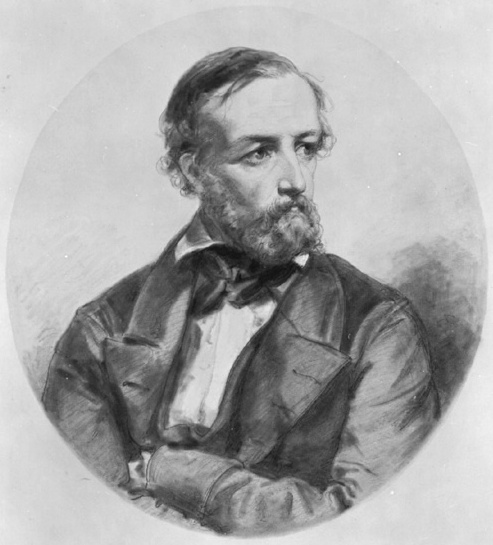
\includegraphics[width=\linewidth]{figures/dirichlet.jpg}
    \captionof*{figure}{\tiny P.G.L. Dirichlet}
  \end{minipage}
  \hfill
  \begin{minipage}[b]{0.45\textwidth}
    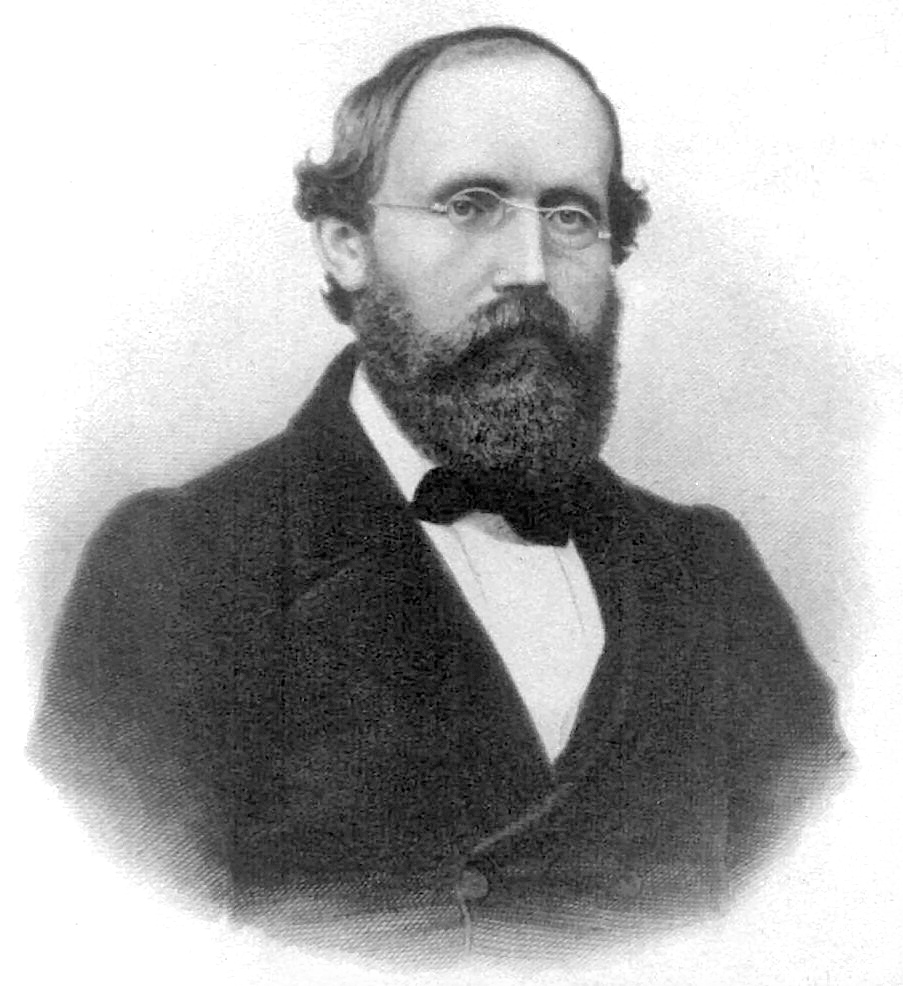
\includegraphics[width=\linewidth]{figures/riemann.jpg}
    \captionof*{figure}{\tiny B. Riemann}
  \end{minipage}
\end{figure}
    \end{minipage}
\end{frame}

\begin{frame}\frametitle{Dirichlet's Principle: Modern Form}
% We seek a minimizer $u$ of the energy functional:
% \begin{equation*}
% 	E(v)
% 	=
% 	\frac{1}{2}
% 	\int_\Omega |\nabla v|^2 \dd x
% 	-
% 	\int_\Omega v f \dd x
% 	\,,
% \end{equation*}
% over the \textbf{closed convex cone} defined by  
% \[
% K = \{ v \in H^1_0(\Omega) \mid v \geq 0 \text{~a.e.}\}.
% \] 
% (Displacements $v \ge 0$, the obstacle)

 \begin{beamercolorbox}[rounded=true, shadow=true, wd=\textwidth]{block body}
\visible<1->{For any $f\in L^2(\Omega)$ and $g\in H^{1/2}(\Gamma)$, the (weak) solution of Poisson's equation over an open bounded Lipschitz domain $\Omega \subset \mathbb{R}^n$ with boundary $\Gamma$
 \begin{equation}
 \label{eq:PoissonEquation}\tag{Poisson Problem}
 	-\Delta u = f
 	\quad \text{in~} \Omega,
 	\qquad
 	u = g \quad \text{on~} \Gamma,
 \end{equation}}\visible<2->{
 is the \textbf{$H^1(\Omega)$-minimizer} of the total energy functional,
 \begin{equation}
 \label{eq:DirichletEnergy}\tag{Dirichlet Energy}
 	E(v)
 	=
 	\frac{1}{2}
 	\int_\Omega |\nabla v|^2 \dd x
 	-
 	\int_\Omega v f \dd x
 	\,,
 \end{equation}}\visible<3->{
 when confined to the \textbf{constraint set} $H^1_g(\Omega) = g + H^1_0(\Omega) = \{ v \in H^1(\Omega) \mid v = g \text{~on~} \partial \Omega\}$.}
\end{beamercolorbox}

\visible<4->{
 \begin{beamercolorbox}[rounded=true, shadow=true, wd=\textwidth]{block title}\centering
 We sketch the proof. The arguments extend to much more complicated examples!
 \end{beamercolorbox}
}
\end{frame}

\begin{frame}\frametitle{The Direct Method}

 \begin{beamercolorbox}[rounded=true, shadow=true, wd=\textwidth]{block body}
 There are a few basic steps
 \begin{enumerate}
 \item Start with a minimizing sequence $\left\{v_k\right\}$ meaning  \[\inf_{v \in H^1_g(\Omega)} E(v) = \liminf_{k \to +\infty} E(v_k).\] 
 \item For some topology $\tau$, show $\left\{v_k\right\}$ admits a $\tau$-convergent subsequence $\left\{v_{k_l}\right\}$ to some $\bar{v}$.
 \item Argue that $\bar{v}$ is a feasible point, i.e. $\bar{v} \in H^1_g(\Omega)$.
 \item Show that $E$ is $\tau$-lower semicontinuous. 
 \end{enumerate}
 \end{beamercolorbox}

\visible<2->{
 \begin{beamercolorbox}[rounded=true, shadow=true, wd=\textwidth]{block title}
% This works because
  \[
 \inf_{v \in H^1_g(\Omega)} E(v) = \liminf_{k \to +\infty} E(v_k) =  \liminf_{l \to +\infty} E(v_{k_l}) \ge E(\bar{v}) \ge  \inf_{v \in H^1_g(\Omega)} E(v).
 \]
  \end{beamercolorbox}}
 
\end{frame}

\begin{frame}\frametitle{The Direct Method}
 \begin{beamercolorbox}[rounded=true, shadow=true, wd=\textwidth]{block body}
 \visible<1->{We would like to \alert{prove} the existence of a solution to the optimization problem:
 \[
 \inf_{u \in H^1_g(\Omega)} E(u).
 \]
We use the \alert{Direct Method of the Calculus of Variations}. For simplicity $g \equiv 0$, $f \ne 0$.}
 \end{beamercolorbox}
 
 \visible<2->{
  \begin{beamercolorbox}[rounded=true, shadow=true, wd=\textwidth]{block body}
% \begin{enumerate}
% \item 
\visible<2->{$E$ is not bound from below here. However,}
\visible<3->{for any $v \in H^1_0(\Omega)$, $E(v)$ is finite and 
 \[
 E(v) \ge \frac{1}{2} \| \nabla v \|^2_{L^2} - \| v \|_{L^2} \|f\|_{L^2} \ge \frac{1}{2} \| \nabla v \|^2_{L^2} - C \|\nabla v \|_{L^2} \| f \|_{L^2}
 \]}\vspace*{-1ex}
% \item 

 \visible<4->{This means, if $\|v\|_{H^1_0} \to +\infty$, then $E(v) \to +\infty$, i.e., $E$ is \alert{$H^1_0(\Omega)$-coercive}.\medskip
% \item 
 }
 
 \visible<5->{
 Thus, $N_0 := \left\{ v \in H^1_0(\Omega) \left| E(v) \le E(v_0) \right.\right\}$ for any $v_0 \in H^1_0(\Omega)$ is \alert{bounded in $H^1_0(\Omega)$}.}
% \end{enumerate}
 \end{beamercolorbox}
 }
\end{frame}

\begin{frame}\frametitle{The Direct Method}
 \visible<1->{\begin{beamercolorbox}[rounded=true, shadow=true, wd=\textwidth]{block body}
\visible<1->{If  $\{v_k\} \subset H^1_0(\Omega)$ is a minimizing sequence, then $v_k \in N_0$ for large $k$.\medskip

Thus, $\{v_k\}$ is a \alert{bounded sequence}.\medskip
}

\visible<2->{$H^1_0(\Omega)$ is Hilbert $\Rightarrow$ bounded sequences admit \alert{weakly convergent subsequences}.\medskip

\visible<3->{Hence, there exists $\{v_{k_l}\} \subset \{v_k\}$ and $\bar{v} \in H^1_0(\Omega)$ such that $v_{k_l} \rightharpoonup \bar{v}$ (weakly in $H^1_0(\Omega))$.

\rule{\linewidth}{0.4pt}\medskip

}


\visible<4->{
$E$ is the sum of a convex continuous function and a continuous linear functional.\medskip
}

\visible<5->{
 We can thus easily show that $E$ is \alert{weakly lower-semicontinuous}, meaning
 \[
 \forall \{v_k\} \subset H^1_0(\Omega) : v_k \rightharpoonup v \quad\text{ we have }\quad \liminf_{k \to +\infty} E(v_k) \ge E(v).
 \]
}\vspace{-2ex}

\visible<6->{
This completes the proof, i.e., $u = \bar{v}$ is a minimizer of $E$ over $H^1_0(\Omega)$.
}
}
 \end{beamercolorbox}
 }
\end{frame}

\begin{frame}\frametitle{Optimality Conditions}
 \visible<1->{\begin{beamercolorbox}[rounded=true, shadow=true, wd=\textwidth]{block body}
  \visible<1->{The objective $E$ is \alert{strongly convex}: There is a $c > 0$ for all $u,v \in H^1_0(\Omega)$ and $\lambda \in [0,1]$
  \[
  E(\lambda u + (1-\lambda) v) \le \lambda E(u) + (1-\lambda) E(v) - c \lambda (1 - \lambda) \| u - v \|^2_{H^1_0}.
  \]
  }\vspace{-2ex}
  
  \visible<2->{
  This makes it easy to show that the minimzer of $E$ is unique. But where's the PDE?
  }\medskip
  
 \visible<3->{
 Observe: 
 \begin{enumerate}
 \item \visible<3->{
  For $v, w \in H^1_g(\Omega)$, $\lambda \in (0,1)$, we have $( \lambda v + (1-\lambda) w)|_{\Gamma} = \lambda g + (1-\lambda) g = g$.
  \item This means the feasible set $H^1_g(\Omega)$ is convex. (Easy to show $\ne\emptyset$ and closed).
 }
\item \visible<4->{
 For any $v \in H^1_g(\Omega)$ and $\tau > 0$ we have 
 \[
 E( u + \tau v) = E(u) + \tau [(\nabla u, \nabla v)_{L^2} - (f,v)_{L^2}] + \frac{\tau^2}{2} \| \nabla v \|^2_{L^2}
 \]
 }\vspace{-3ex}
 \end{enumerate}
 }
 \end{beamercolorbox}}
\end{frame}

\begin{frame}\frametitle{Optimality Conditions}
 \visible<1->{\begin{beamercolorbox}[rounded=true, shadow=true, wd=\textwidth]{block body}
 Consider the definition of our unique minimizer $u$: 
 \[
 E(u) \le E(v) \quad \forall v \in H^1_g(\Omega).
 \]
 
 \visible<2->{
 Since $H^1_g(\Omega)$ is a convex set, $\lambda v + (1-\lambda) u = u + \lambda (v - u) \in H^1_g(\Omega)$ for all $v \in H^1_g(\Omega)$.
 }\medskip
 
  \visible<3->{
  Then for fixed arbitrary $v \in H^1_g(\Omega)$, we have:
  \[
  E(u) \le E(u + \lambda (v - u) ) = E(u) + \lambda [(\nabla u, \nabla [v-u])_{L^2} - (f,v-u)_{L^2}] + \frac{\lambda^2}{2} \| \nabla [v-u] \|^2_{L^2}
  \]
  and hence,
  \[
 \lambda [(\nabla u, \nabla [v-u])_{L^2} - (f,v-u)_{L^2}] \ge o(\lambda) 
  \]
  Divide by $\lambda > 0$ and let $\lambda \to 0$.
  }
 
 \end{beamercolorbox}}
\end{frame}

\begin{frame}\frametitle{A First Variational Inequality}
 \visible<1->{\begin{beamercolorbox}[rounded=true, shadow=true, wd=\textwidth]{block body}
 \visible<1->{The following \alert{variational inequality} characterizes our solution $u$:
 \[
 (\nabla u, \nabla [v-u])_{L^2} \ge  (f,v-u)_{L^2} \quad \forall v \in H^1_g(\Omega)
 \]
 It states: \textit{The direction derivative of $E$ at $u$ in any feasible direction $v - u$ is non-negative.}
 }\medskip
 
\visible<2->{
In this simple example, we have, for any $v \in H^1_g(\Omega)$ and $w \in H^1_0(\Omega)$, $v + w \in H^1_g(\Omega)$.
}\medskip
 
\visible<3->{
This means $u \in H^1_g(\Omega)$ solves
 \[
 (\nabla u, \nabla w)_{L^2} =  (f,w)_{L^2} \quad \forall v \in H^1_0(\Omega),
 \]
 which brings us back to Poisson. (use $u + w$ and $u-w$ in the VI)
 }
  \end{beamercolorbox}}
  
\visible<4->{\begin{beamercolorbox}[rounded=true, shadow=true, wd=\textwidth]{block title}
\centering  But what about more complicated feasible sets?
\end{beamercolorbox}}
\end{frame}

\section{Elliptic Variational Inequalities}

\begin{frame}{Elliptic Variational Inequalities}
        \begin{enumerate}
        \item A slight twist on Dirichlet's principle
            \begin{enumerate}
                \item Conic constraint ($u \ge 0$)
                \item Follow Dirichlet above for derivation
            \end{enumerate}
        \item A second variational inequality: An obstacle problem
        \item A brief history of variational inequalities (of the first kind)
        \item The Lions-Stampacchia theorem
        \item Mignot's theorem
            \begin{enumerate}
                \item 
            \end{enumerate}
    \end{enumerate}
\end{frame}

\begin{frame}{Elliptic Variational Inequalities}
 \visible<1->{\begin{beamercolorbox}[rounded=true, shadow=true, wd=\textwidth]{block body}
Given $u \in H^1(\Omega)$ with $u|_{\Gamma} = g$ we look for solutions satisfying a \alert{pointwise inequality}:
 \[
  u \ge \varphi \quad \text{almost everywhere (a.e.) on } \Omega.
 \]
 Denote this \alert{feasible set} by $K$.
 \end{beamercolorbox}}
\end{frame}

\section{Examples}\label{sec:examples}
\begin{frame}{Examples of Variational Inequalities}
    \begin{enumerate}
        \item Signorini problem
        \item Stefan problem
        \item Black-Scholes
        \item Multiphase phase transition
        \item Elastoplastic torsion
        \item Ice sheet
        \item Diffusive wave equation
    \end{enumerate}
\end{frame}
\section{Alternative Formulations}\label{sec:complementarity}
\begin{frame}{A Complementarity Formulation}
        \begin{enumerate}
        \item Derivation of a complementarity problem
        \item Regularity of the multiplier
        \item Active, Inactive, and Biactive sets
        \item General form of multiplier?
    \end{enumerate}
\end{frame}
\section{Solution Algorithms}\label{sec:algorithms}
\begin{frame}{Algorithms}
    \begin{enumerate}
        \item Penalty
        \item Barrier
        \item Augmented Lagrangian
    \end{enumerate}
\end{frame}


% \begin{frame}{Frame Title}
    
% \end{frame}
% \begin{frame}{Frame Title}
    
% \end{frame}
% \begin{frame}{Frame Title}
    
% \end{frame}
% \begin{frame}{Frame Title}
    
% \end{frame}
% \section{}
% \begin{frame}{Frame Title}
    
% \end{frame}
% \begin{frame}{Frame Title}
    
% \end{frame}
% \begin{frame}{Frame Title}
    
% \end{frame}
% \begin{frame}{Frame Title}
    
% \end{frame}
% \begin{frame}{Frame Title}
    
% \end{frame}
% \section{}
% \begin{frame}{Frame Title}
    
% \end{frame}
% \begin{frame}{Frame Title}
    
% \end{frame}
% \begin{frame}{Frame Title}
    
% \end{frame}
% \begin{frame}{Frame Title}
    
% \end{frame}

\end{document}